\documentclass[12pt,letterpaper,noanswers]{exam}
\usepackage[usenames,dvipsnames,svgnames,table]{xcolor}
\usepackage[margin=0.9in]{geometry}
\renewcommand{\familydefault}{\sfdefault}
\usepackage{multicol}
\pagestyle{head}
\header{AM 108 Class 24}{}{Maps}
\runningheadrule
\headrule
\usepackage{graphicx} % more modern
\usepackage{amsmath} 
\usepackage{amssymb} 
\usepackage{hyperref}
\usepackage{tcolorbox}

\begin{document}
 \pdfpageheight 11in 
  \pdfpagewidth 8.5in

\noindent 




\begin{itemize}
\item No problem set: project work this week.
\item There is a skill check for Friday.
\item There is a discussion board post summary due Friday.
\end{itemize}

\hrule
\vspace{0.2cm}



\noindent\textbf{Project Teams}

Team 1: Jessica, Coco, Isaac G.

Team 2: Emily, Justin, Zhao (spread of political ideas)

Team 3: Annabelle, Laura, Winnie

Team 4: Daniel, Isaac A, Jaleel (inequality in society, education)

Team 5: Dabao, Mark, Charlie (biology / patterning)

Team 6: Martin, Hal

Team 7: Ethan (will join Team 6 during class today)

Zhe will join team 6 during class today.


\noindent \textbf{Teams 3 and 4}: Post screenshots of your work to the course Google Drive today.  Include words, labels, and other short notes that might make those solutions useful to you or your classmates.  Find the link in Canvas (or here: \url{https://drive.google.com/drive/u/0/folders/1GcpwvKHD4tMecpFQ4lNxN_r5Ylj7YHbd})


\vspace{0.2cm}

\hrule
\vspace{0.2cm}


\noindent\textbf{Big picture}

The Lorenz '63 system is an important example of a system with sensitive dependence on initial conditions.  We saw that one way to represent a trajectory of that system is via the Lorenz map.

We also learned about the logistic map, which is smooth (unlike the Lorenz map) and will serve as a model system for exploring one route to chaos.
\vspace{0.2cm}
\hrule
\vspace{0.2cm}

\noindent \textbf{Extra vocabulary / extra facts:}
\begin{tcolorbox}
The \textbf{Lorenz `map'} is constructed from a list of local maxima of $z(t)$ for a single trajectory of the Lorenz system.  We plot $z_{n+1}$ vs $z_n$ to represent the map.  Think of this map as telling us our next local maximum value of $z$ given our current local maximum value.  This is not really a map: there is some thickness to the curve.  We will treat it like a map, however.

A \textbf{fixed point} of a map $x_{n+1} = f(x_n)$ occurs when $x = f(x)$.

A fixed point of a map is \textbf{stable} when $-1 < f'(x) < 1$.

In the context of a map, the value $f'(x^*)$ is called a \textbf{multiplier}.

The \textbf{orbit} of a point is the set $\{x_0, x_1, x_2, ...\}$ where $x_n$ is formed under the action of the map.

The map $x_{n+1} = rx(1-x)$ is known as the \textbf{logistic map}.

The map $x_{n+1} = \left\{\begin{array}{c c}2x_n & 0\leq x_n \leq 1/2 \\ 2-2x_n & 1/2 \leq x_n \leq 1 \end{array} \right.$ is an example of a \textbf{tent map}.
\end{tcolorbox}

\vspace{0.2cm}
\hrule
\vspace{0.2cm}

\noindent\textbf{Your questions}
\begin{enumerate}
    \item Lorenz map
    \begin{enumerate}
        \item Do $x_n$ and $y_n$ produce similar maps, or just $z_n$?
        \item If we see a map that is similar to the Lorenz map, can we conclude we are working with the Lorenz system?
        \item When would we use this kind of map to understand an attractor?
        \item What are the exceptions to $z$ that will be on the Lorenz map?
        \item For the stability of the periodic orbit, why did we use $z^*= f(z^*)$?
        \item How do we know $f'(z^*)>1$ for the fixed point of the Lorenz map?
        \item Steve suggested there could be periodic orbits of the Lorenz map.  How would we determine their stability?
        \item How do we reconcile the existence of the attractor with the fact that the system is dissipative, so the limiting set would have no volume?
    \end{enumerate}
    \item Logistic map
    \begin{enumerate}
        \item What are the ranges of $r$ for which we will see different kinds of behavior in the logistic map?
        \item There is a stable period-3 cycle around $r= 3.83$.  Would we then period-double based on the period-3 cycle?
    \end{enumerate}
\end{enumerate}

The `map', for a trajectory integrated to time $5000$:

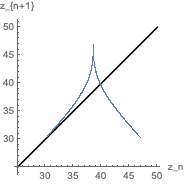
\includegraphics{img/191104-C25p1.png}

Trajectories near the fixed point: On the left, $x$ is in blue, $y$ in orange, and $z$ in green for $10$ time units starting at a time very close to the fixed point.  On the right, the trajectory is plotted in $3$-space.

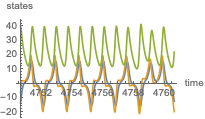
\includegraphics{img/191104-C25p2.png}
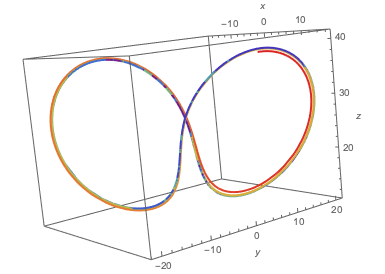
\includegraphics[width=0.4\textwidth]{img/191104-C25p3.png}

\vspace{0.2cm}
\hrule
\vspace{0.2cm}

\noindent\textbf{Skill Check C25 practice}
\begin{questions}
\item Retake of skill check C22: separation of two trajectories.

\item A map has a period-2 orbit with $1.7 = f(1.2)$ and $1.2 = f(1.7)$ with $f'(1.2) = 0.3$ and $f'(1.7) = 1.2$.

Using linear stability (so considering the  multiplier for the map $x_{n+2} = g(x_n) = f(f(x_n))$, identify the stability of the period-2 orbit.

\end{questions}

\vspace{0.2cm}

\hrule
\vspace{0.2cm}

\noindent\textbf{Skill check C25 practice solution}

Think of the two points in the period-$2$ orbit as $p$ and $q$, with $p = f(q)$ and $q = f(p)$

Write our map as $x_{n+2} = g(x_n)$, where our function $g$ is $f(f(x))$.  The multiplier is given by $\left.g'\right\vert_{x=q} = \left.f'(f(x))f'(x)\right\vert_{x=q}$ by the chain rule.  Substituting for $p = f(q)$ this becomes $g'(q) = f'(p)f'(q)$.  That means the stability of the 2-cycle is given by the product of the slopes at the two points involved in the 2-cycle (note that this generalizes to k-cycles...).  $f'(p) = 0.3$ and $f'(q) = 1.7$ so $g'(q) = f'(p)f'(q) = 0.3*1.7 = $ uh...

3*17 = 21+30 = 51 and I need to put in the decimals, so I get $0.51$.  That is less than $1$ in magnitude, so this 2-cycle is stable.


\vspace{0.2cm}

\hrule
\vspace{0.2cm}
\noindent\textbf{Questions}

\noindent \ \ 0.  Share whatever you would like, and write your names on the slide.

\begin{questions}

\question
Consider the map $x_{n+1} = 3.25 x_n(1-x_n) = f(x_n)$.  This is a logistic map ($r = 3.25$).

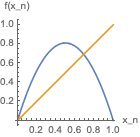
\includegraphics{img/191104-C25p4.png}
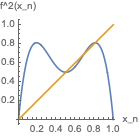
\includegraphics{img/191104-C25p4b.png}

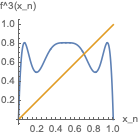
\includegraphics{img/191104-C25p4c.png}
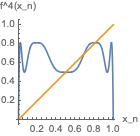
\includegraphics{img/191104-C25p4d.png}


\begin{parts}
\item The map $x_{n+1} = f(x_n)$ has a fixed point.  Find it on the plots above and approximate it using a numerical tool.  Identify its stability by comparing $f'(x^*)$ to $1$.
\item A \textbf{period-2 orbit} occurs when there is a point $p$ such that $f(p) = q$ and $f(q) = p$, so $f(f(p)) = p$.  This can be written $f^2(p) = p$.  So a period-2 orbit shows up as a fixed points of $x_{n+2} = f^2(x_n)$.
\begin{itemize}
\item Look at the graph of $f(f(x_n))$ above.  How many fixed points does it have?  How many period-2 orbits does it have?
\item To find the stability of a period-2 orbit, we consider $\lambda = \frac{d}{dx} f(f(p))$ where the point $p$ is a point in the period-2 orbit.  This is $f'(f(p))f'(p)$.  Show that $f'(f(p))f'(p) = f'(f(q))f'(q)$ where $q$ is the other point in the orbit.
\item Find $\lambda = \frac{d}{dx} f(f(p))$ for the map above and compare its magnitude to $1$.  Is the period-2 orbit stable or unstable?
\item Is there a period-3 orbit in this system?  Use the appropriate plot above.
\item What about a period-4 orbit?  Use the appropriate plot above.  What is causing there to be fixed points in this plot?
\end{itemize}
\end{parts}


\question (9.4.2) The tent map is a simple analytical model that has some properties in common with the Lorenz map.
Let \[
x_{n+1} = \left\{
        \begin{array}{ll}
            2x_n, & \quad 0\leq x_n \leq \frac{1}{2} \\
            2-2x_n, & \quad \frac{1}{2}\leq x_n \leq 1.
        \end{array}
    \right.
    \]
    \begin{parts}
    \item Draw $f(x)$ where $x_{n+1} = f(x_n)$.  How many times does it intersect the curve $y=x$?  Why is this map the ``tent map''?
    \item Find the fixed points of this map.
    \item Classify the stability of the fixed points.
    \item Sketch the graph of $f(f(x))$.  How many times does it intersect the curve $y = x$?
    \item Show the map has a period-$2$ orbit.  This means that there is an $x$ such that $f(f(x)) = x$ (but $f(x)\neq x$).
    \item Classify the stability of any period-$2$ orbits.
    \item Look for a period-$3$ or period-$4$ point.  If you find one, are such orbits stable or unstable?
    \item If you want, you can think about whether there is a period-$k$ orbit...
    \end{parts}


\end{questions}

\eject

\begin{enumerate}
\item the fixed points happens when the orange line and the blue curve intersect.  0.7 something, it looks like.  Also $x = 0$.
\begin{verbatim}
Solve[x == 3.25 x (1 - x), x]
D[3.25 x (1 - x), x] /. x -> 0.6923
\end{verbatim}
Mathematica gives me $x \approx 0.6923$ for the fixed point.
For stability, I'm getting a multiplier of $\approx -1.25$, so unstable.

b: There are four fixed points where $f(f(x))=x$.  Two of them are fixed points of $f$ (since those will also be fixed in $f(f(x))$).  Two are fixed in $f(f(x))$.  That's actually just one period-2 orbit, though, because if $p\rightarrow q \rightarrow p$ then $f(f(p)) = p$ and $f(f(q))=q$.

\begin{verbatim}
f[x_] := 3.25 x (1 - x);
fp = Solve[x == f[f[x]], x]
D[f[f[x]], x] /. fp
\end{verbatim}

The multiplier is $\approx -0.0625$, so the period-2 orbit is stable ($-1 < \text{multiplier} < 1$

To think about period $3$, we look at the $f(f(f(x)))$ plot.  It has two fixed points, which came from $ x= f(x)$, so these are period-1 fixed points, not period-3 ones and there's no period-3 orbit.

For period-4, we're seeing the period 1 and period 2 show up but nothing new, so there isn't a period-4 orbit either.

\item
\begin{enumerate}
\item  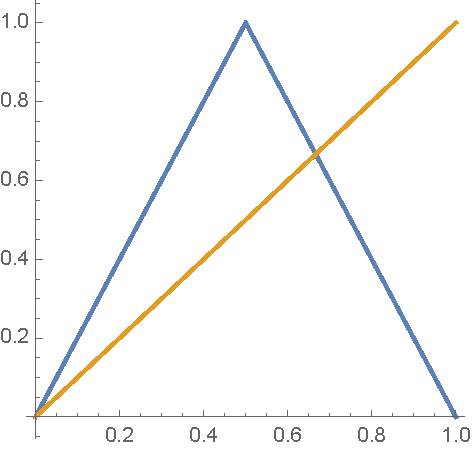
\includegraphics[scale=0.5]{img/C20map1.pdf} 

Two intersections, so two fixed points.
\item If $2x = x$ then $ x = 0$, so $0$ is a fixed point.  If $2 -2 x = x$ then $2 - 3x = 0$ so 
$x = \frac{2}{3}$.  $\frac{1}{2}\leq \frac{2}{3}\leq 1$, so $\frac{2}{3}$ is also a fixed point.  Looking at the graph of this below,
there are two intersections between $y=f(x)$ and $y=x$ corresponding to two fixed points.
\item

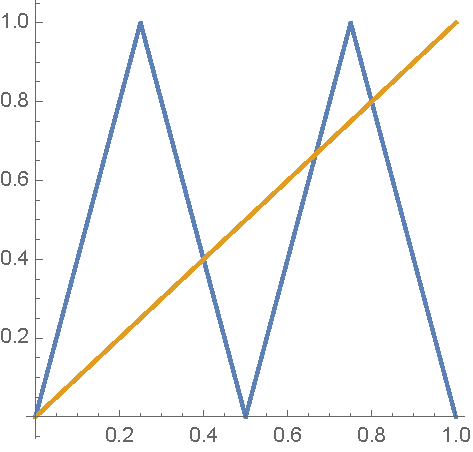
\includegraphics[scale=0.5]{img/C20map2.pdf}

It intersects the curve four times.  Two of these are the fixed points from above where $x^* = f(x^*) = f(f(x^*))$.  Two of them are points where $x_0 = x_2$ but $x_0 \neq x_1$.  We call those two points $p$ and $q$.  So $p = f(q) = f(f(p))$.
\item $\frac{df}{dx} = \pm 2$ so it is greater than $1$ in magnitude.  This means the fixed points are unstable.
\item $x = f(f(x))$.  If $0\leq x\leq \frac{1}{2}$ then $x \rightarrow 2x$.  If $0\leq x \leq \frac{1}{4}$ then $x \rightarrow 2x \rightarrow 4x$.
This has a fixed point of $0$ but that isn't a period $2$ point.  If $\frac{1}{4} \leq x \leq \frac{1}{2}$ then $x \rightarrow 2x \rightarrow 2 - 4x$.
This has a fixed point of $x = 2 - 4x$ so $x = \frac{2}{5}$.  $f(\frac{2}{5}) = \frac{4}{5}$ so the period-$2$ orbit is 
$x_1=\frac{2}{5}, x_2=\frac{4}{5}.$

Looking at the graph of $y=f(f(x))$ below, there are $4$ intersection points with $y=x$.  These correspond
 to the two period-$1$ fixed points and two new
fixed points.  The two new fixed points form a period-$2$ orbit.
\item For the stability, we created the map explicitly, so it is clear that $x_{n+2} = f(f(x_n))$ has a Floquet multiplier of $4$, and is
unstable.  More generally,
thinking about the growth of a perturbation near the period-$2$ point, let $z_n$ be a point near the period-2 orbit and let $\eta_n$
be the distance of $z_n$ from the orbit.  $\eta_{n+2} \approx f'(z_{n+1})\eta_{n+1} \approx f'(z_{n+1})f'(z_n)\eta_n$.  In our case,
$\vert f'(z) \vert = 2$ for all $z$, so $\vert f'(z_{n+1})f'(z_n) \vert = 4$.
\item From above, any such orbit is unstable.  Now, can we find one?  For the period-$3$, looking at the $y=f(f(f(x)))$ graph below,
there are six intersection points.  Two of these correspond to the period-$1$ points.  The other $6$ are new and correspond to two
different period-$3$ orbits ($\frac{2}{9},...$ and $\frac{2}{7}...$.)  

The map for period-$4$ should have $2^4=16$ intersections, of which two are period-$1$ and two are period-$2$ but the other $12$
should be new, so $3$ period-$4$ orbits.
\begin{figure}[h]
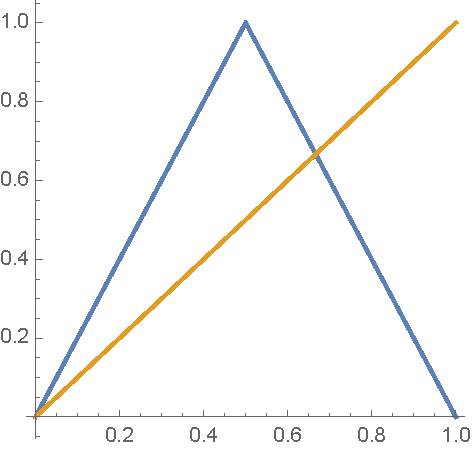
\includegraphics[scale=0.5]{img/C20map1.pdf}
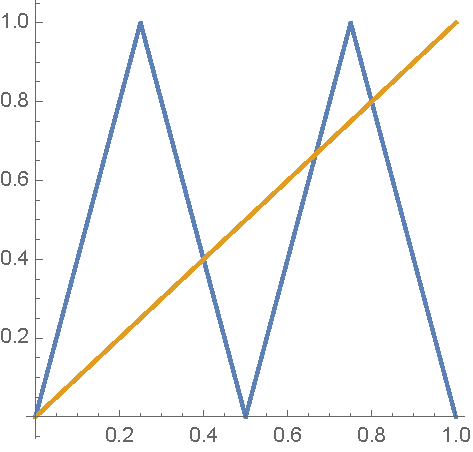
\includegraphics[scale=0.5]{img/C20map2.pdf}
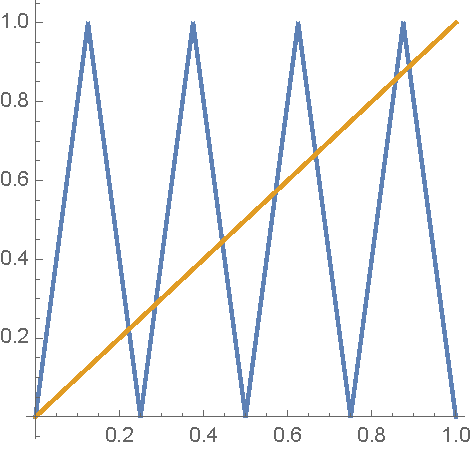
\includegraphics[scale=0.5]{img/C20map3.pdf}
\caption{Maps from left: $x_{n+1} = f(x_n)$, $x_{n+2} = f(f(x_n))$ and $x_{n+3} = f(f(f(x_n)))$.}
\end{figure}

\end{enumerate}
\end{enumerate}

\end{document}